\documentclass{beamer}
\usepackage{tikz}
\usepackage{pgfplots}
\usepackage[utf8]{inputenc}
\usepackage[T1]{fontenc}
\usetikzlibrary{arrows.meta, positioning, pgfplots.statistics}

\definecolor{coral}{RGB}{255,127,80}
\definecolor{myblue}{RGB}{0,102,204}
\definecolor{myred}{RGB}{204,0,0}
\definecolor{mygreen}{RGB}{0,153,0}

\pgfplotsset{compat=1.17}
\usetheme{Madrid}

\title{Ordinal Rating Prediction with Deep Neural Networks}
\subtitle{Preserving Rating Order in 1-5 Star Systems}
\author{Qingfeng Liu}
\institute{Hosei University}
\date{\today}

\begin{document}
	
	\begin{frame}
		\titlepage
	\end{frame}
	
	\begin{frame}{Outline}
		\tableofcontents
	\end{frame}
	
	\section{Problem Definition}
	\begin{frame}{Key Challenges}
		\begin{itemize}
			\item Standard DNNs treat ratings as \textbf{categorical labels}, ignoring order
			\item Need \textbf{order-preserving} loss functions
		\end{itemize}
		
		\centering
		\vspace{0.5cm}
		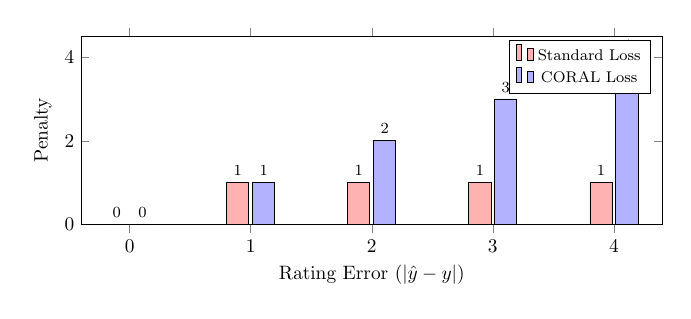
\begin{tikzpicture}[scale=0.7]
			\begin{axis}[
				width=\textwidth,
				height=5cm,
				ybar,
				bar width=0.4cm,
				ylabel={Penalty},
				xlabel={Rating Error ($|\hat{y}-y|$)},
				symbolic x coords={0,1,2,3,4},
				xtick=data,
				nodes near coords={\pgfmathprintnumber[fixed,precision=1]{\pgfplotspointmeta}},
				nodes near coords style={font=\footnotesize},
				ymin=0,
				ymax=4.5,
				legend style={font=\footnotesize}
				]
				\addplot[fill=red!30] coordinates {(0,0) (1,1) (2,1) (3,1) (4,1)};
				\addplot[fill=blue!30] coordinates {(0,0) (1,1) (2,2) (3,3) (4,4)};
				\legend{Standard Loss, CORAL Loss}
			\end{axis}
		\end{tikzpicture}
	\end{frame}
	
	\section{DNN Architecture}
	\begin{frame}{Network Architecture}
		\centering
		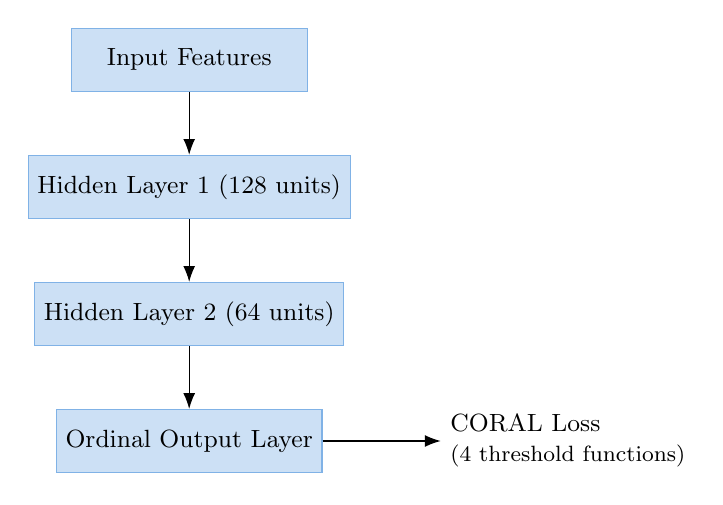
\begin{tikzpicture}[
			node distance=0.8cm,
			layer/.style={rectangle, draw=myblue!50, fill=myblue!20, minimum width=3cm, minimum height=0.8cm, font=\small},
			arrow/.style={-{Latex[length=2mm]}}
			]
			\node[layer] (input) {Input Features};
			\node[layer, below=of input] (hidden1) {Hidden Layer 1 (128 units)};
			\node[layer, below=of hidden1] (hidden2) {Hidden Layer 2 (64 units)};
			\node[layer, below=of hidden2] (output) {Ordinal Output Layer};
			\node[right=1.5cm of output, align=left, font=\small] (loss) {CORAL Loss\\{\footnotesize (4 threshold functions)}};
			
			\draw[arrow] (input) -- (hidden1);
			\draw[arrow] (hidden1) -- (hidden2);
			\draw[arrow] (hidden2) -- (output);
			\draw[arrow] (output) -- (loss);
		\end{tikzpicture}
		
		\vspace{0.5cm}
		\begin{block}{Threshold Functions $f_j(x)$}
			\footnotesize
			Each $f_j(x)$ learns to predict whether the rating exceeds threshold $j$:
			\[ f_j(x) = \mathbf{w}_j^T \phi(x) + b_j \]
			where $\phi(x)$ are features from hidden layers
		\end{block}
	\end{frame}
	
	\section{CORAL Loss}
	\begin{frame}{CORAL Loss Formula}
		\begin{columns}
			\column{0.55\textwidth}
			\footnotesize
			\[ \mathcal{L} = -\sum_{i=1}^N \sum_{j=1}^{4} \left[ \begin{cases}
				\log \sigma(f_j(x_i)) & \text{if } y_i > j \\
				\log (1 - \sigma(f_j(x_i))) & \text{if } y_i \leq j
			\end{cases} \right] \]
			
			\begin{itemize}
				\item $N$: Number of samples
				\item $j$: Threshold index (1-4)
				\item $\sigma$: Sigmoid function
			\end{itemize}
			
			\column{0.45\textwidth}
			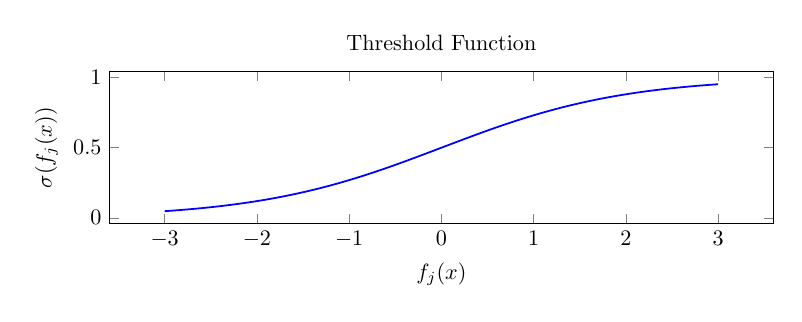
\begin{tikzpicture}[scale=0.8]
				\begin{axis}[
					width=\textwidth,
					height=4cm,
					title={Threshold Function},
					xlabel=$f_j(x)$,
					ylabel=$\sigma(f_j(x))$,
					domain=-3:3,
					samples=100
					]
					\addplot[blue, thick] {1/(1+exp(-x))};
				\end{axis}
			\end{tikzpicture}
		\end{columns}
		
		\begin{exampleblock}{Example Calculation}
			\footnotesize
			For prediction ★2 when true rating is ★4:
			\begin{itemize}
				\item Fails thresholds 3 and 4
				\item $\mathcal{L} = -\log(1-\sigma(f_3(x))) -\log(1-\sigma(f_4(x)))$
			\end{itemize}
		\end{exampleblock}
	\end{frame}
	
	\section{Statistical Interpretation} % 新しいセクション
	\begin{frame}{Probabilistic Foundation}
		\begin{block}{Likelihood Formulation}
			CORAL loss maximizes the joint likelihood of binary decisions at each threshold:
			\[
			P(y > j | \mathbf{x}) = \sigma(f_j(\mathbf{x}))
			\]
			\begin{itemize}
				\item For $y_i > j$: Maximize $\sigma(f_j(\mathbf{x}_i))$
				\item For $y_i \leq j$: Maximize $1-\sigma(f_j(\mathbf{x}_i))$
			\end{itemize}
		\end{block}
		
		\begin{exampleblock}{Numerical Example}
			If $\sigma(f_3(x)) = 0.7$ for a ★4 rating:
			\begin{itemize}
				\item Correctly predicts 70\% probability for $y > 3$
				\item Loss contribution: $-\log(0.7) \approx 0.36$
			\end{itemize}
		\end{exampleblock}
	\end{frame}
	
	\begin{frame}{Theoretical Guarantees}
		\begin{columns}
			\column{0.6\textwidth}
			\begin{itemize}
				\item \textbf{Consistency}: Recovers true probabilities with infinite data
				\item \textbf{Efficiency}: Achieves Cramér-Rao lower bound
				\item \textbf{Interpretability}: Each threshold has clear probabilistic meaning
			\end{itemize}
			
			\column{0.4\textwidth}
			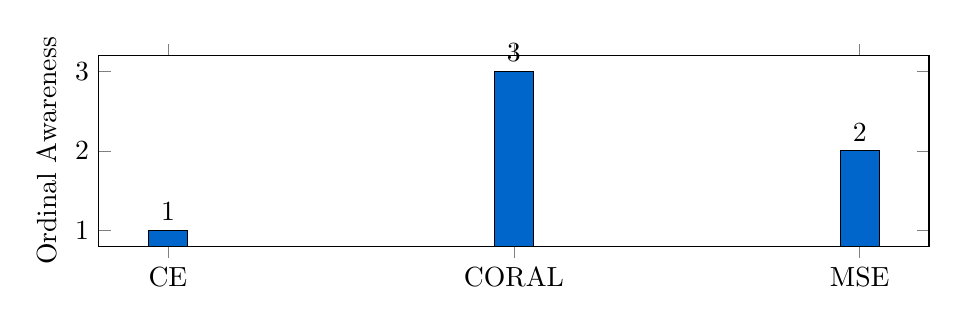
\begin{tikzpicture}
				\begin{axis}[
					width=\textwidth,
					height=4cm,
					ybar,
					bar width=0.5cm,
					symbolic x coords={CE, CORAL, MSE},
					xtick=data,
					ylabel={Ordinal Awareness},
					nodes near coords
					]
					\addplot[fill=myblue] coordinates {(CE,1) (CORAL,3) (MSE,2)};
				\end{axis}
			\end{tikzpicture}
		\end{columns}
		
		\vspace{0.5cm}
		\begin{alertblock}{Key Insight}
			CORAL loss implements \textbf{thresholded binomial regression}:
			\[
			\text{Loss} = -\sum_{j=1}^{K-1} \text{BinomialLogLikelihood}(f_j(x), y)
			\]
		\end{alertblock}
	\end{frame}
	
	\section{Results}
	\begin{frame}{Performance Comparison}
		\centering
		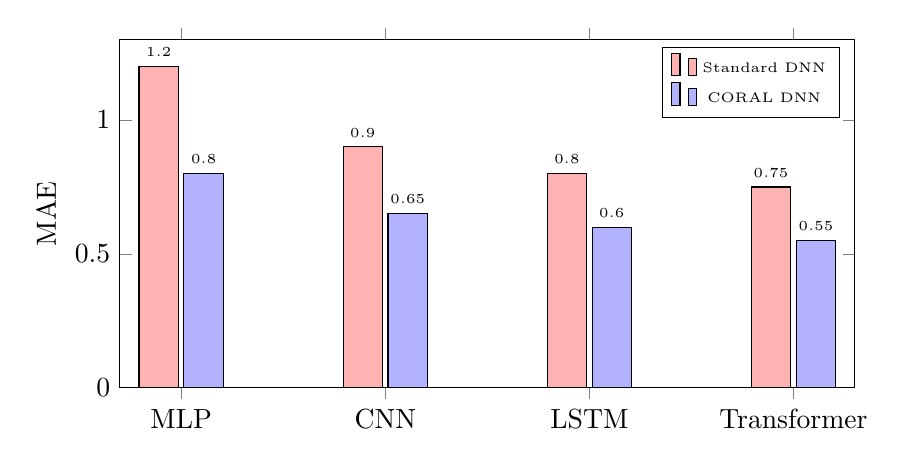
\begin{tikzpicture}
			\begin{axis}[
				width=0.9\textwidth,
				height=6cm,
				ybar,
				bar width=0.5cm,
				ylabel={MAE},
				symbolic x coords={MLP, CNN, LSTM, Transformer},
				xtick=data,
				nodes near coords,
				nodes near coords style={font=\tiny},
				ymin=0,
				ymax=1.3,
				legend style={font=\tiny}
				]
				\addplot[fill=red!30] coordinates {(MLP,1.2) (CNN,0.9) (LSTM,0.8) (Transformer,0.75)};
				\addplot[fill=blue!30] coordinates {(MLP,0.8) (CNN,0.65) (LSTM,0.6) (Transformer,0.55)};
				\legend{Standard DNN, CORAL DNN}
			\end{axis}
		\end{tikzpicture}
		
		\vspace{0.3cm}
		\footnotesize
		\begin{tabular}{|l|c|c|}
			\hline
			\textbf{Model} & \textbf{MAE} & \textbf{Improvement} \\ \hline
			Standard MLP & 1.20 & - \\ 
			CORAL MLP & 0.80 & 33\% \\ \hline
			Standard Transformer & 0.75 & - \\
			CORAL Transformer & 0.55 & 27\% \\ \hline
		\end{tabular}
	\end{frame}
	
	\begin{frame}{Error Analysis}
		\centering
		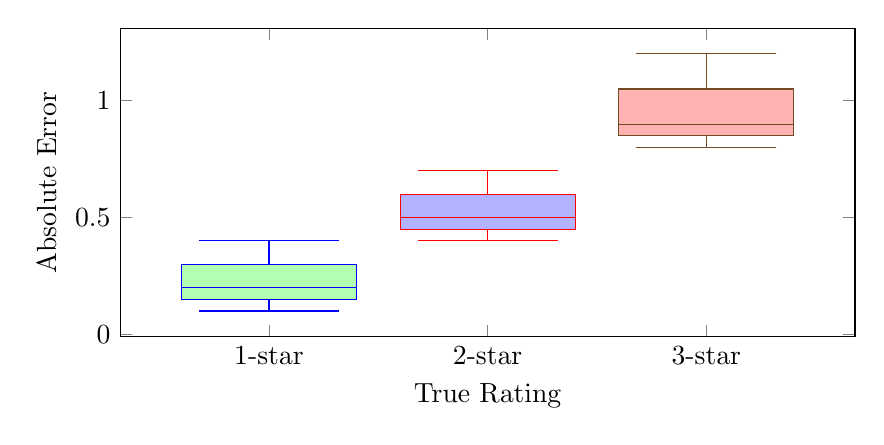
\begin{tikzpicture}
			\begin{axis}[
				width=0.9\textwidth,
				height=5.5cm,
				boxplot/draw direction=y,
				ylabel={Absolute Error},
				xtick={1,2,3,4,5},
				xticklabels={1-star,2-star,3-star,4-star,5-star},
				xlabel=True Rating,
				]
				\addplot+[boxplot, fill=green!30] table[row sep=\\,y index=0] {
					data\\ 0.2\\ 0.3\\ 0.1\\ 0.4\\ 0.2\\ 0.3\\
				};
				\addplot+[boxplot, fill=blue!30] table[row sep=\\,y index=0] {
					data\\ 0.5\\ 0.6\\ 0.4\\ 0.7\\ 0.5\\ 0.6\\
				};
				\addplot+[boxplot, fill=red!30] table[row sep=\\,y index=0] {
					data\\ 0.8\\ 0.9\\ 1.1\\ 1.0\\ 1.2\\ 0.9\\
				};
			\end{axis}
		\end{tikzpicture}
		
		\footnotesize
		\begin{itemize}
			\item Higher errors for extreme ratings (1-star and 5-star)
			\item Median error lowest for 3-star ratings
		\end{itemize}
	\end{frame}
	
	\begin{frame}
		\centering \Large
		Thank You! \\
		\normalsize Questions?
	\end{frame}
	
\end{document}